\documentclass[aspectratio=169]{beamer}
\usepackage{graphicx}
\usepackage{float}
\usepackage{textpos}
\usepackage{subcaption}
\usepackage{hyperref}
\usepackage{booktabs}
\usepackage{tikz}
\usetikzlibrary{shapes.geometric, arrows.meta, positioning}
\newcommand{\angstrom}{\text{\normalfont\AA}}
\usetheme{CambridgeUS}
\author{Shen Wang}
\institute{The Ohio State University}
\title{AI for Research Workshop}
\titlegraphic{
	\begin{textblock}{3}(12,0.5)
	
\includegraphics[scale=0.2]{logo_OSU.png}
	\end{textblock}}

\date{October 15, 2025}
\begin{document}
\frame{\titlepage}

\begin{frame}{Outline}

\vspace{0.5cm}
\Large

\begin{itemize}
\setlength{\itemsep}{0.4cm}

\item \textbf{Model Context Protocol (MCP)}
\item \textbf{Subagents \& Automation}
\item \textbf{GitHub Integration \& Best Practices}

\end{itemize}

\end{frame}

\begin{frame}{Model Context Protocol (MCP)}

\vspace{0.3cm}
\centering
\large
MCP is an open-source standard that connects AI applications to external systems.

\vspace{0.5cm}

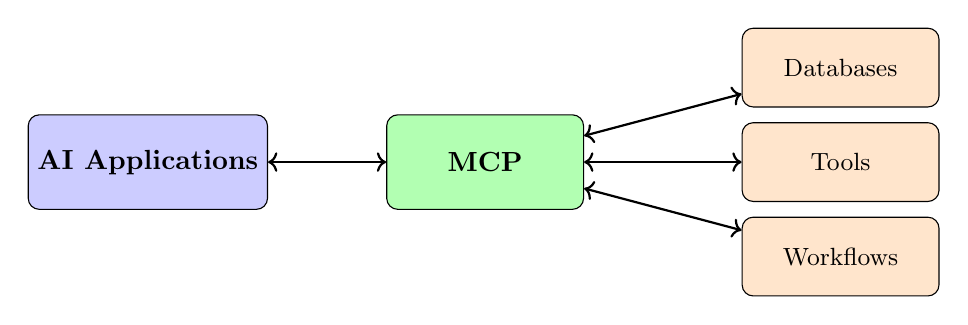
\begin{tikzpicture}[
    node distance=2cm,
    box/.style={rectangle, rounded corners, minimum width=2.5cm, minimum height=1.2cm, text centered, draw=black, fill=blue!20, font=\normalsize\bfseries},
    protocol/.style={rectangle, rounded corners, minimum width=2.5cm, minimum height=1.2cm, text centered, draw=black, fill=green!30, font=\normalsize\bfseries},
    resource/.style={rectangle, rounded corners, minimum width=2.5cm, minimum height=1cm, text centered, draw=black, fill=orange!20, font=\small},
    arrow/.style={-{Stealth[length=3mm]}, thick}
]

% AI Applications
\node[box] (ai) {AI Applications};

% MCP Protocol
\node[protocol, right=1.5cm of ai] (mcp) {MCP};

% Resources
\node[resource, right=2cm of mcp, yshift=1.2cm] (db) {Databases};
\node[resource, right=2cm of mcp] (tools) {Tools};
\node[resource, right=2cm of mcp, yshift=-1.2cm] (workflows) {Workflows};

% Arrows
\draw[arrow, <->] (ai) -- (mcp);
\draw[arrow, <->] (mcp) -- (db);
\draw[arrow, <->] (mcp) -- (tools);
\draw[arrow, <->] (mcp) -- (workflows);

\end{tikzpicture}

\end{frame}

\begin{frame}

\vspace{0.5cm}
\centering
\Large
\textbf{AI agents need tools — just like humans use calculators}

\vspace{1cm}

\begin{columns}[t]

\column{0.3\textwidth}
\centering
\textbf{\large Real-time Data}
\vspace{0.4cm}

\normalsize
\begin{itemize}
\item Weather forecasts
\item Current search results
\item Up-to-date information
\end{itemize}

\column{0.3\textwidth}
\centering
\textbf{\large Taking Action}
\vspace{0.4cm}

\normalsize
\begin{itemize}
\item Modify files
\item Send emails
\item Schedule meetings
\end{itemize}

\column{0.3\textwidth}
\centering
\textbf{\large Specialized Expertise}
\vspace{0.4cm}

\normalsize
\begin{itemize}
\item Molecular modeling
\item Scientific computing
\item Literature databases
\end{itemize}

\end{columns}

\end{frame}

\begin{frame}

\vspace{2cm}
\centering
\Huge
\textbf{PyMOL-MCP Demo}

\end{frame}

\begin{frame}

\vspace{1cm}
\centering
\Large

MCP tools are like API calls or function definitions

\vspace{1cm}

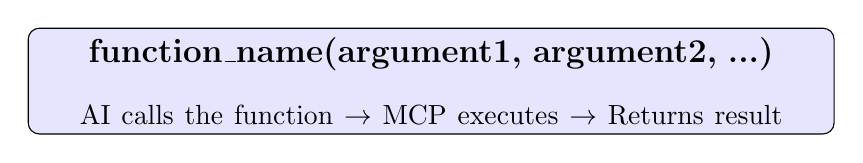
\begin{tikzpicture}
\node[rectangle, draw, rounded corners, fill=blue!10, text width=10cm, align=center, font=\large] {
\textbf{function\_name(argument1, argument2, ...)}\\
\vspace{0.3cm}
\normalsize
AI calls the function $\rightarrow$ MCP executes $\rightarrow$ Returns result
};
\end{tikzpicture}

\vspace{1cm}

\large
\textbf{Key insight:} Anything with an API can become MCP tools

\end{frame}



\begin{frame}[fragile]{Original: One MCP Tool per PyMOL Command}

\vspace{0.1cm}
\small
Each PyMOL function becomes a separate MCP tool with specific arguments:

\vspace{0.2cm}

\begin{verbatim}
@mcp.tool()
def fetch(structure: str):
    """Fetch structure from PDB"""
    return cmd.fetch(structure)

@mcp.tool()
def show(representation: str, selection: str):
    """Show molecular representation"""
    return cmd.show(representation, selection)

@mcp.tool()
def color(color: str, selection: str):
    """Color selection"""
    return cmd.color(color, selection)

... (hundreds more tools)
\end{verbatim}

\vspace{0.1cm}
\normalsize
\textbf{Problem:} Must create one MCP tool for each PyMOL function

\end{frame}

\begin{frame}[fragile]{Modified: Two Generic MCP Tools}

\vspace{0.1cm}
\small
Just 2 MCP tools — AI decides which PyMOL function to call:

\vspace{0.2cm}

\begin{verbatim}
@mcp.tool()
def pymol_command(command: str):
    """Execute any PyMOL command"""
    # AI sends: "fetch 1ubq" or "show cartoon" or "color red, chain A"
    return cmd.do(command)

@mcp.tool()
def pymol_python_api(python_code: str):
    """Execute any PyMOL Python API"""
    # AI sends: "cmd.fetch('1ubq')" or "cmd.align('obj1', 'obj2')"
    return execute(python_code)
\end{verbatim}

\vspace{0.1cm}
\normalsize
\textbf{Same PyMOL API, different MCP interface}\\
\textbf{Advantage:} AI decides which function and arguments to use

\end{frame}

\begin{frame}

\vspace{0.3cm}

\begin{columns}[t]

\column{0.48\textwidth}
\centering
\textbf{\large Original (Community)}
\vspace{0.3cm}

\normalsize
\begin{itemize}
\item Large command dictionary
\item Complex parsing logic
\item Pre-validate all commands
\item Error pattern matching
\item One main tool
\end{itemize}

\vspace{0.5cm}
\textcolor{red}{\textbf{More code, less flexible}}

\column{0.48\textwidth}
\centering
\textbf{\large Modified (Simplified)}
\vspace{0.3cm}

\normalsize
\begin{itemize}
\item No command dictionary
\item Direct execution
\item Two simple tools
\item Let AI formulate commands
\item ~290 lines total
\end{itemize}

\vspace{0.5cm}
\textcolor{blue}{\textbf{Less code, more powerful}}

\end{columns}

\vspace{0.8cm}
\centering
\large
\textbf{Key insight:} AI already knows PyMOL — no need to reinvent the wheel

\end{frame}

\begin{frame}{Building Your Own MCP}

\vspace{0.3cm}
\centering
\Large
\textbf{Anything with an API can become MCP tools}

\vspace{0.5cm}

\begin{columns}[t]

\column{0.48\textwidth}
\centering
\textbf{\large Start Using MCP}
\vspace{0.4cm}

\normalsize
\begin{itemize}
\item Search existing MCP servers
\item github.com/modelcontextprotocol
\item Install and experiment
\item Iterate with AI assistance
\end{itemize}

\column{0.48\textwidth}
\centering
\textbf{\large Build Your Own}
\vspace{0.4cm}

\normalsize
\begin{itemize}
\item Identify API/function to wrap
\item Keep functions simple
\item Let AI handle intelligence
\item AI helps you code it
\end{itemize}

\end{columns}

\vspace{0.8cm}
\centering
\Large
\textbf{Discussion: What APIs would you connect to AI?}

\end{frame}

\begin{frame}{Subagents}

\vspace{0.5cm}
\centering
\Large
Subagents are specialized AI assistants for specific tasks

\vspace{0.8cm}

\normalsize
\begin{itemize}
\item Each subagent has its own separate context window
\item Designed for specific types of tasks (code review, debugging, data analysis)
\item Configurable with custom tools and permissions
\item Can be invoked automatically or explicitly
\end{itemize}

\end{frame}

\begin{frame}

\vspace{0.5cm}
\centering
\Large
\textbf{Complex tasks need specialized experts}

\vspace{1cm}

\begin{columns}[t]

\column{0.3\textwidth}
\centering
\textbf{\large Context Management}
\vspace{0.4cm}

\normalsize
\begin{itemize}
\item Preserve main conversation
\item Isolate complex analysis
\item Return only results
\end{itemize}

\column{0.3\textwidth}
\centering
\textbf{\large Specialized Focus}
\vspace{0.4cm}

\normalsize
\begin{itemize}
\item Custom system prompts
\item Task-specific tools
\item Expert-level execution
\end{itemize}

\column{0.3\textwidth}
\centering
\textbf{\large Efficiency}
\vspace{0.4cm}

\normalsize
\begin{itemize}
\item Parallel task processing
\item Reusable across projects
\item Faster problem-solving
\end{itemize}

\end{columns}

\end{frame}

\begin{frame}

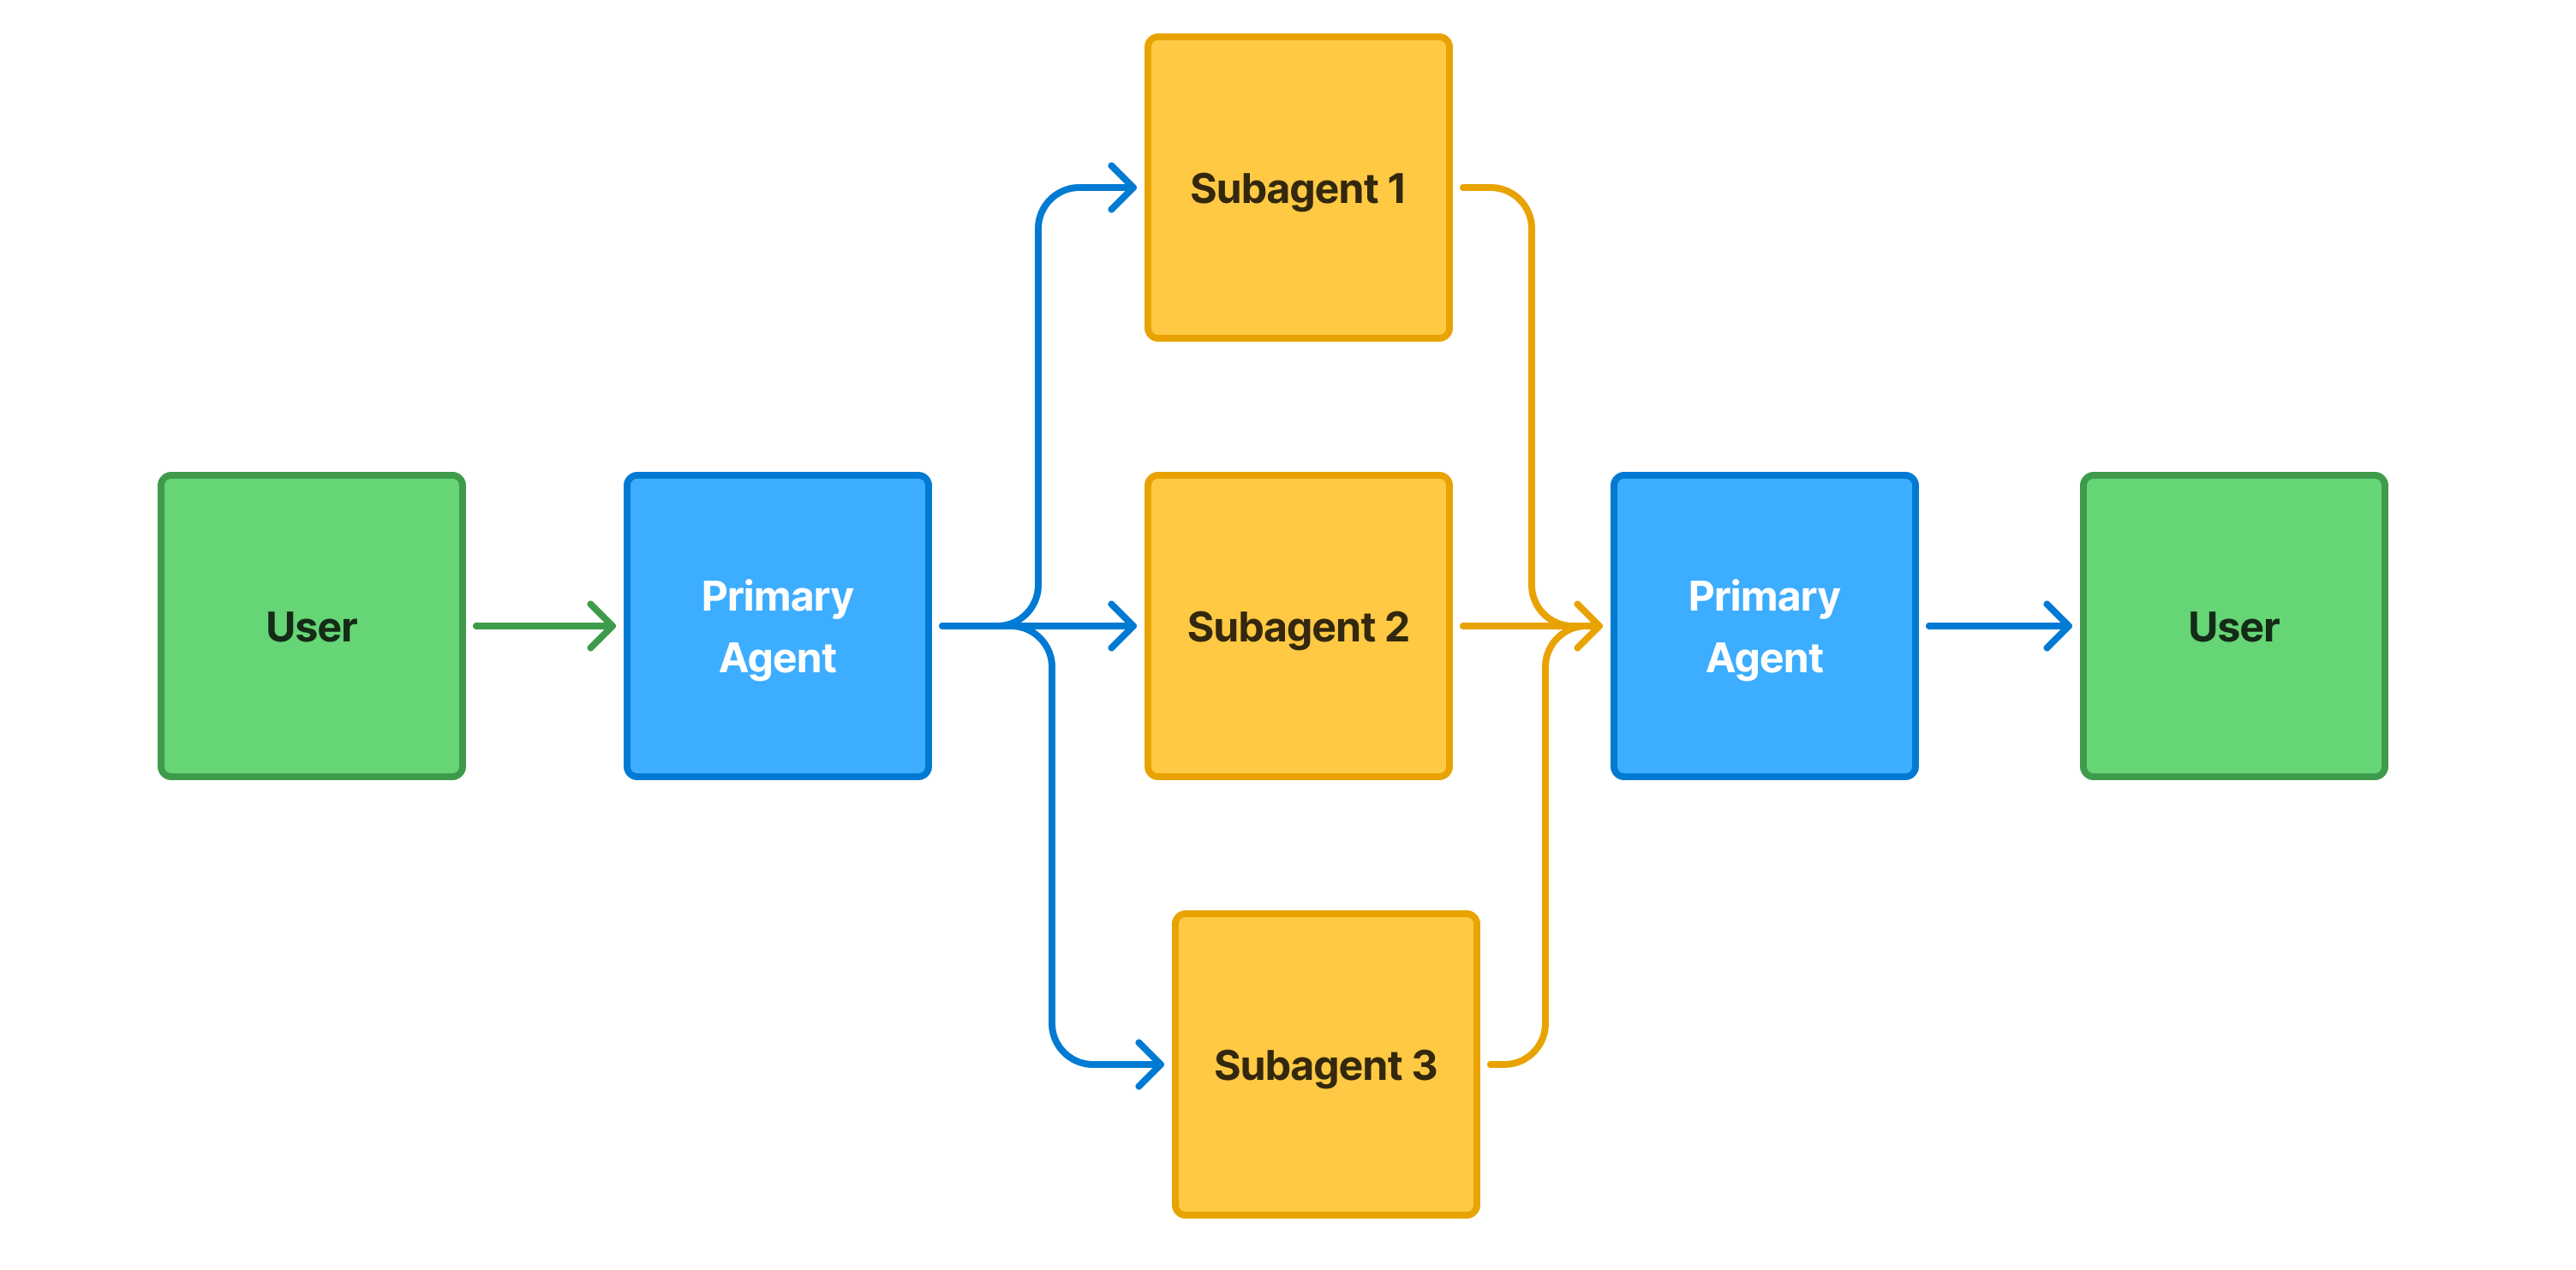
\includegraphics[width=0.9\textwidth]{figures/fig_subagents.png}

{\small
\textbf{Key point:} Subagents communicate only with the primary agent, not directly with users}

\end{frame}



\begin{frame}

\centering

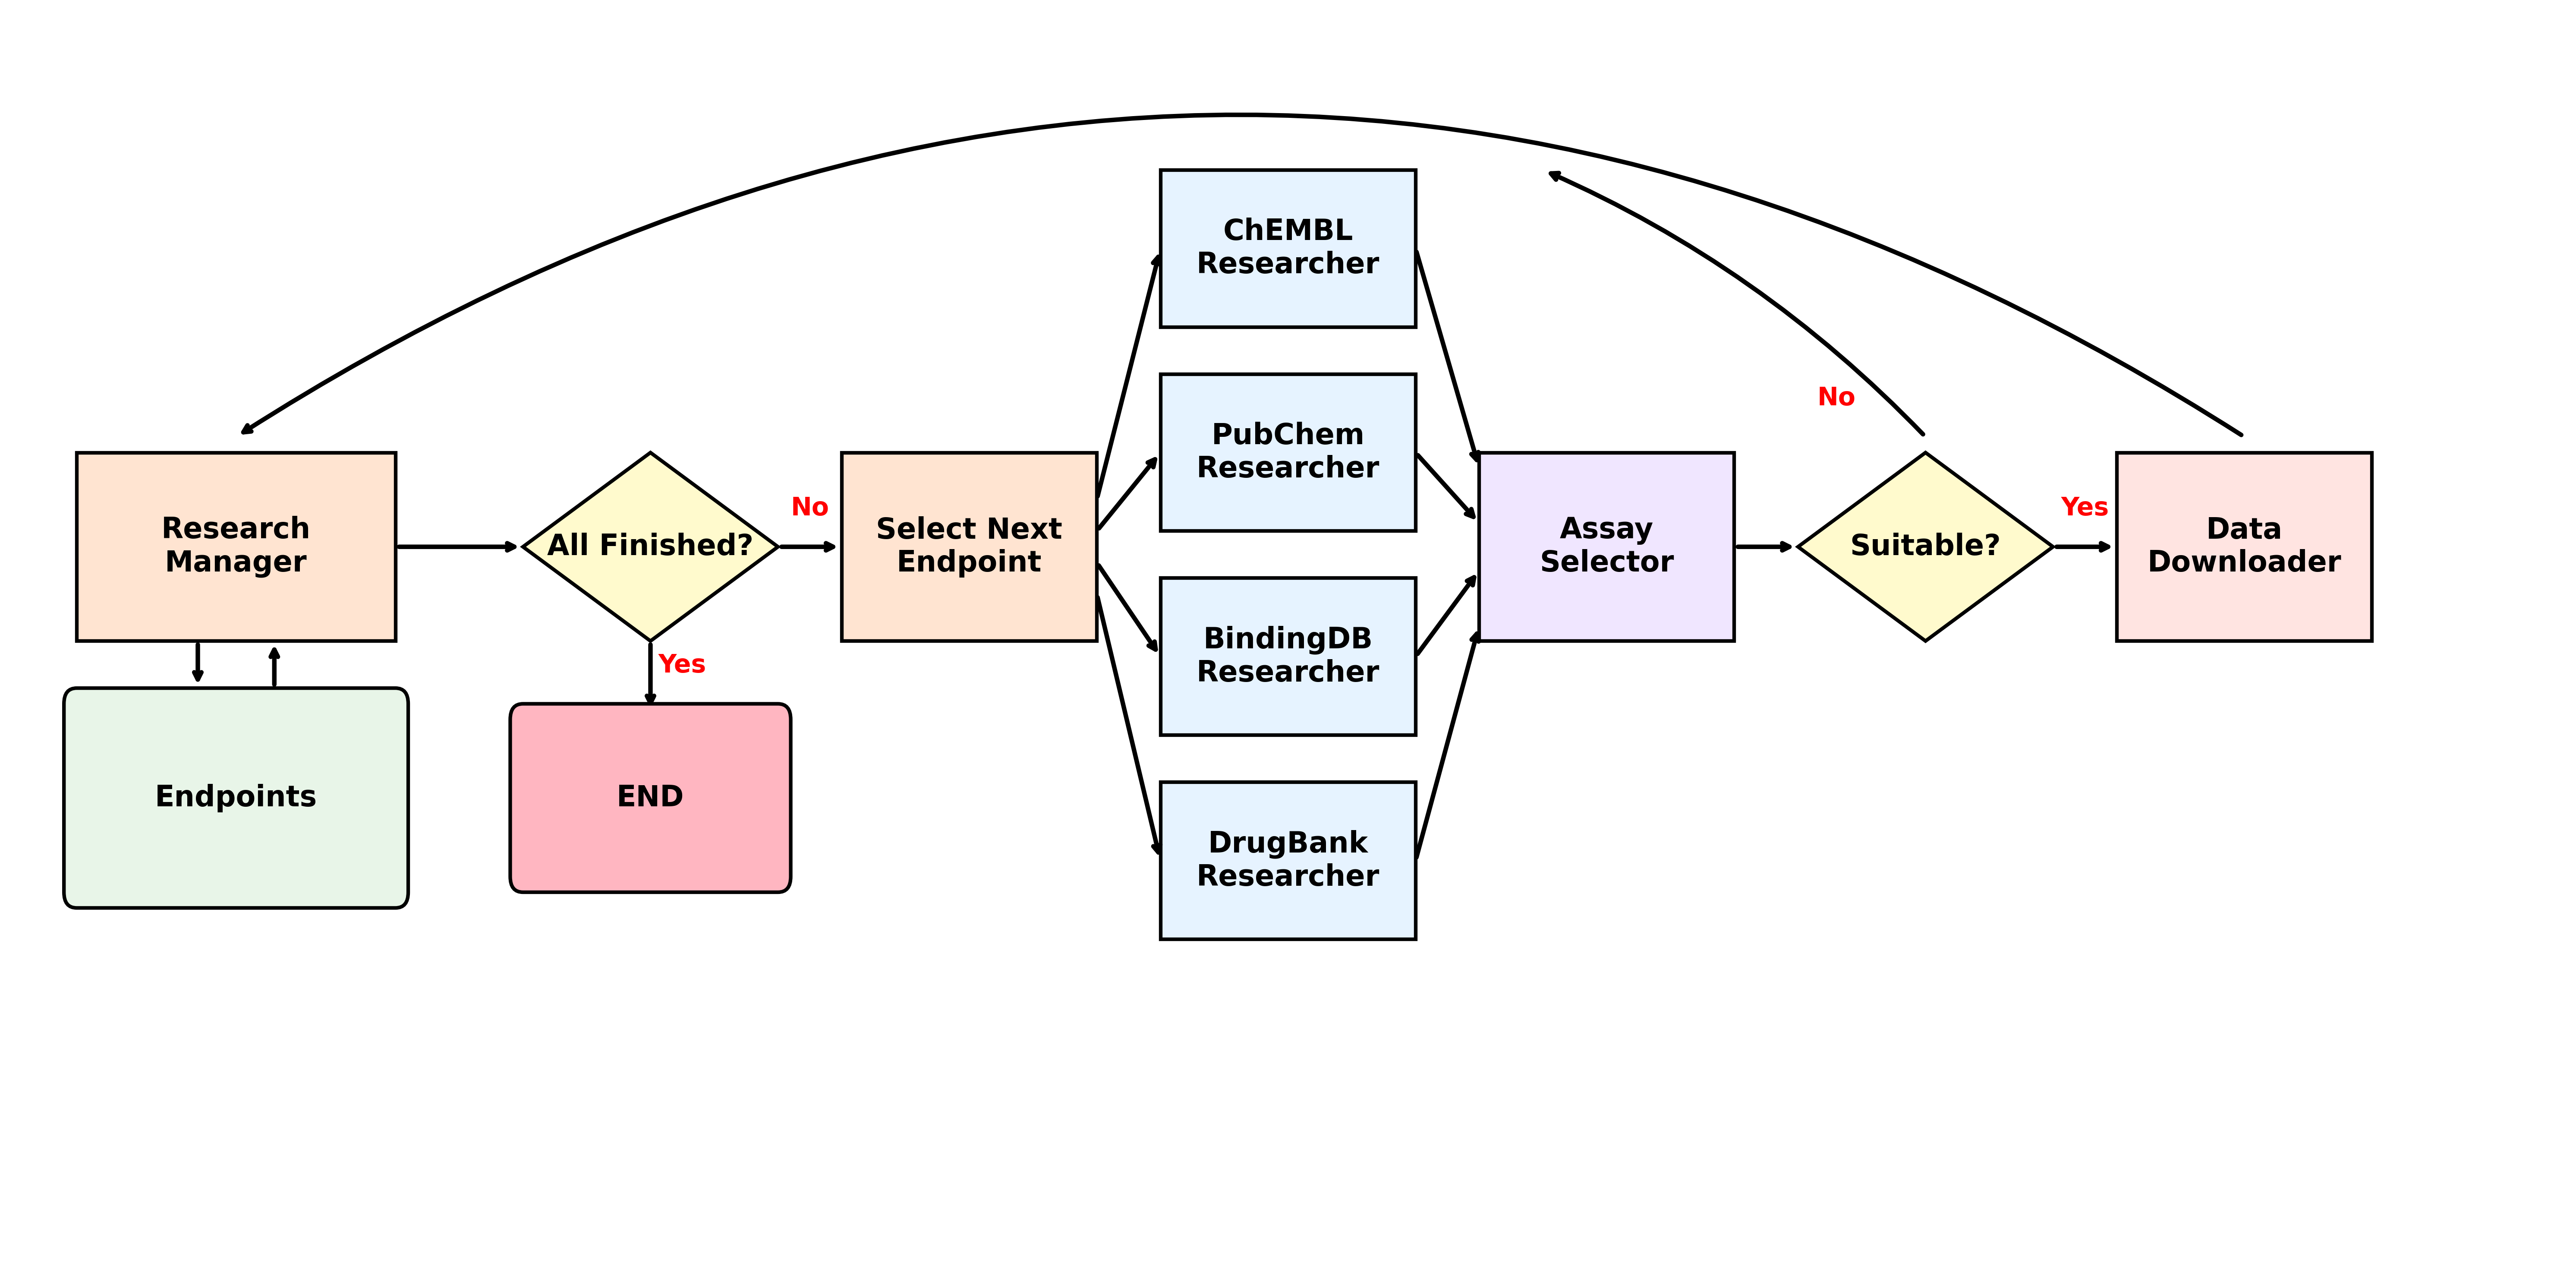
\includegraphics[width=0.95\textwidth]{figures/fig_agent_workflow.png}

\end{frame}

\begin{frame}[fragile]{Creating Your Own Agents with Meta-Agent}

\centering
\begin{columns}[t]


\column{0.48\textwidth}
\centering
\textbf{Configuration Header}

\footnotesize
\begin{verbatim}
---
name: meta-agent
description: Generates new or
  optimizes existing sub-agents
tools: Write, WebFetch,
  MultiEdit, Read, Glob
model: opus
color: cyan
---
\end{verbatim}

\column{0.48\textwidth}
\centering
\textbf{Instructions Workflow}

\footnotesize
\begin{verbatim}
Documentation
  - Fetch latest Anthropic docs

FOR NEW Agent Creation:
  - Analyze requirements
  - Devise name (kebab-case) and Select color & tools
  - Write delegation desc
  - Create system prompt
  - Save to .claude/agents/

OPTIMIZATION:
  - Analyze current config
  - Apply improvements
\end{verbatim}

\end{columns}
\end{frame}

\begin{frame}{Tips for Creating Effective Agents}

\begin{itemize}

\item \textbf{1. Start with documentation fetch}\\
\small It is great to begin by fetching the latest docs — ensures your agent uses current best practices

\item \textbf{2. Define a clear role}\\
\small One specific purpose, one clear responsibility — avoid multi-purpose agents

\item \textbf{3. Define clear input and output}\\
\small \textcolor{blue}{Critical:} Subagents don't communicate with users directly\\
\small Specify exactly what information to return, (A text file report might be helpful)

\item \textbf{4. Use meta-agent to optimize}\\
\small Let meta-agent help refine your prompts and improve agent performance

\end{itemize}
\centering
\vspace{0.6cm}
\Large
\textbf{Discussion: What specialized subagents would help us research?}

\end{frame}

\begin{frame}{Hooks: App-Level Automation}

\vspace{0.5cm}
\centering
\Large
\textbf{Hooks = User-defined commands that run automatically}
\vspace{0.5cm}
\normalsize
\begin{columns}

\column{0.46\textwidth}
\centering
\textbf{\large What Are Hooks?}

\begin{itemize}
\item Shell commands triggered by events
\item Execute at specific points in lifecycle
\item Provide deterministic control
\end{itemize}

\column{0.08\textwidth}
\centering
\rule{1pt}{4cm}

\column{0.46\textwidth}
\centering
\textbf{\large Hook Events}

\begin{itemize}
\item \texttt{PreToolUse} — Before tools run
\item \texttt{PostToolUse} — After tools complete
\item \texttt{UserPromptSubmit} — On user input
\item \texttt{Stop} — When AI finishes
\end{itemize}

\end{columns}
\vspace{0.5cm}
\centering
\large
\textbf{Key insight:} Hooks make Claude Code behavior predictable and customizable

\end{frame}

\begin{frame}{My Essential Hooks}

\vspace{0.3cm}

\begin{itemize}
\setlength{\itemsep}{0.5cm}

\item \textbf{Safety Guard Hook} — \texttt{PreToolUse}
\begin{itemize}
\item Blocks dangerous operations like \texttt{rm -rf} before execution
\item Allows enabling "dangerously mode" without actual risk
\end{itemize}

\item \textbf{Task Completion Notifications} — \texttt{Stop}
\begin{itemize}
\item Plays sound or sends desktop notification when Claude finishes
\item Get alerted when Claude needs your input or review
\end{itemize}

\item \textbf{Git Commit Standards} — \texttt{PreToolUse}
\begin{itemize}
\item Enforces naming conventions for branches and commits
\item Limits commit messages to concise lengths (50-100 chars)
\end{itemize}

\end{itemize}

\vspace{0.4cm}

\end{frame}

\begin{frame}{GitHub Integration Workflow}

\vspace{0.5cm}
\centering
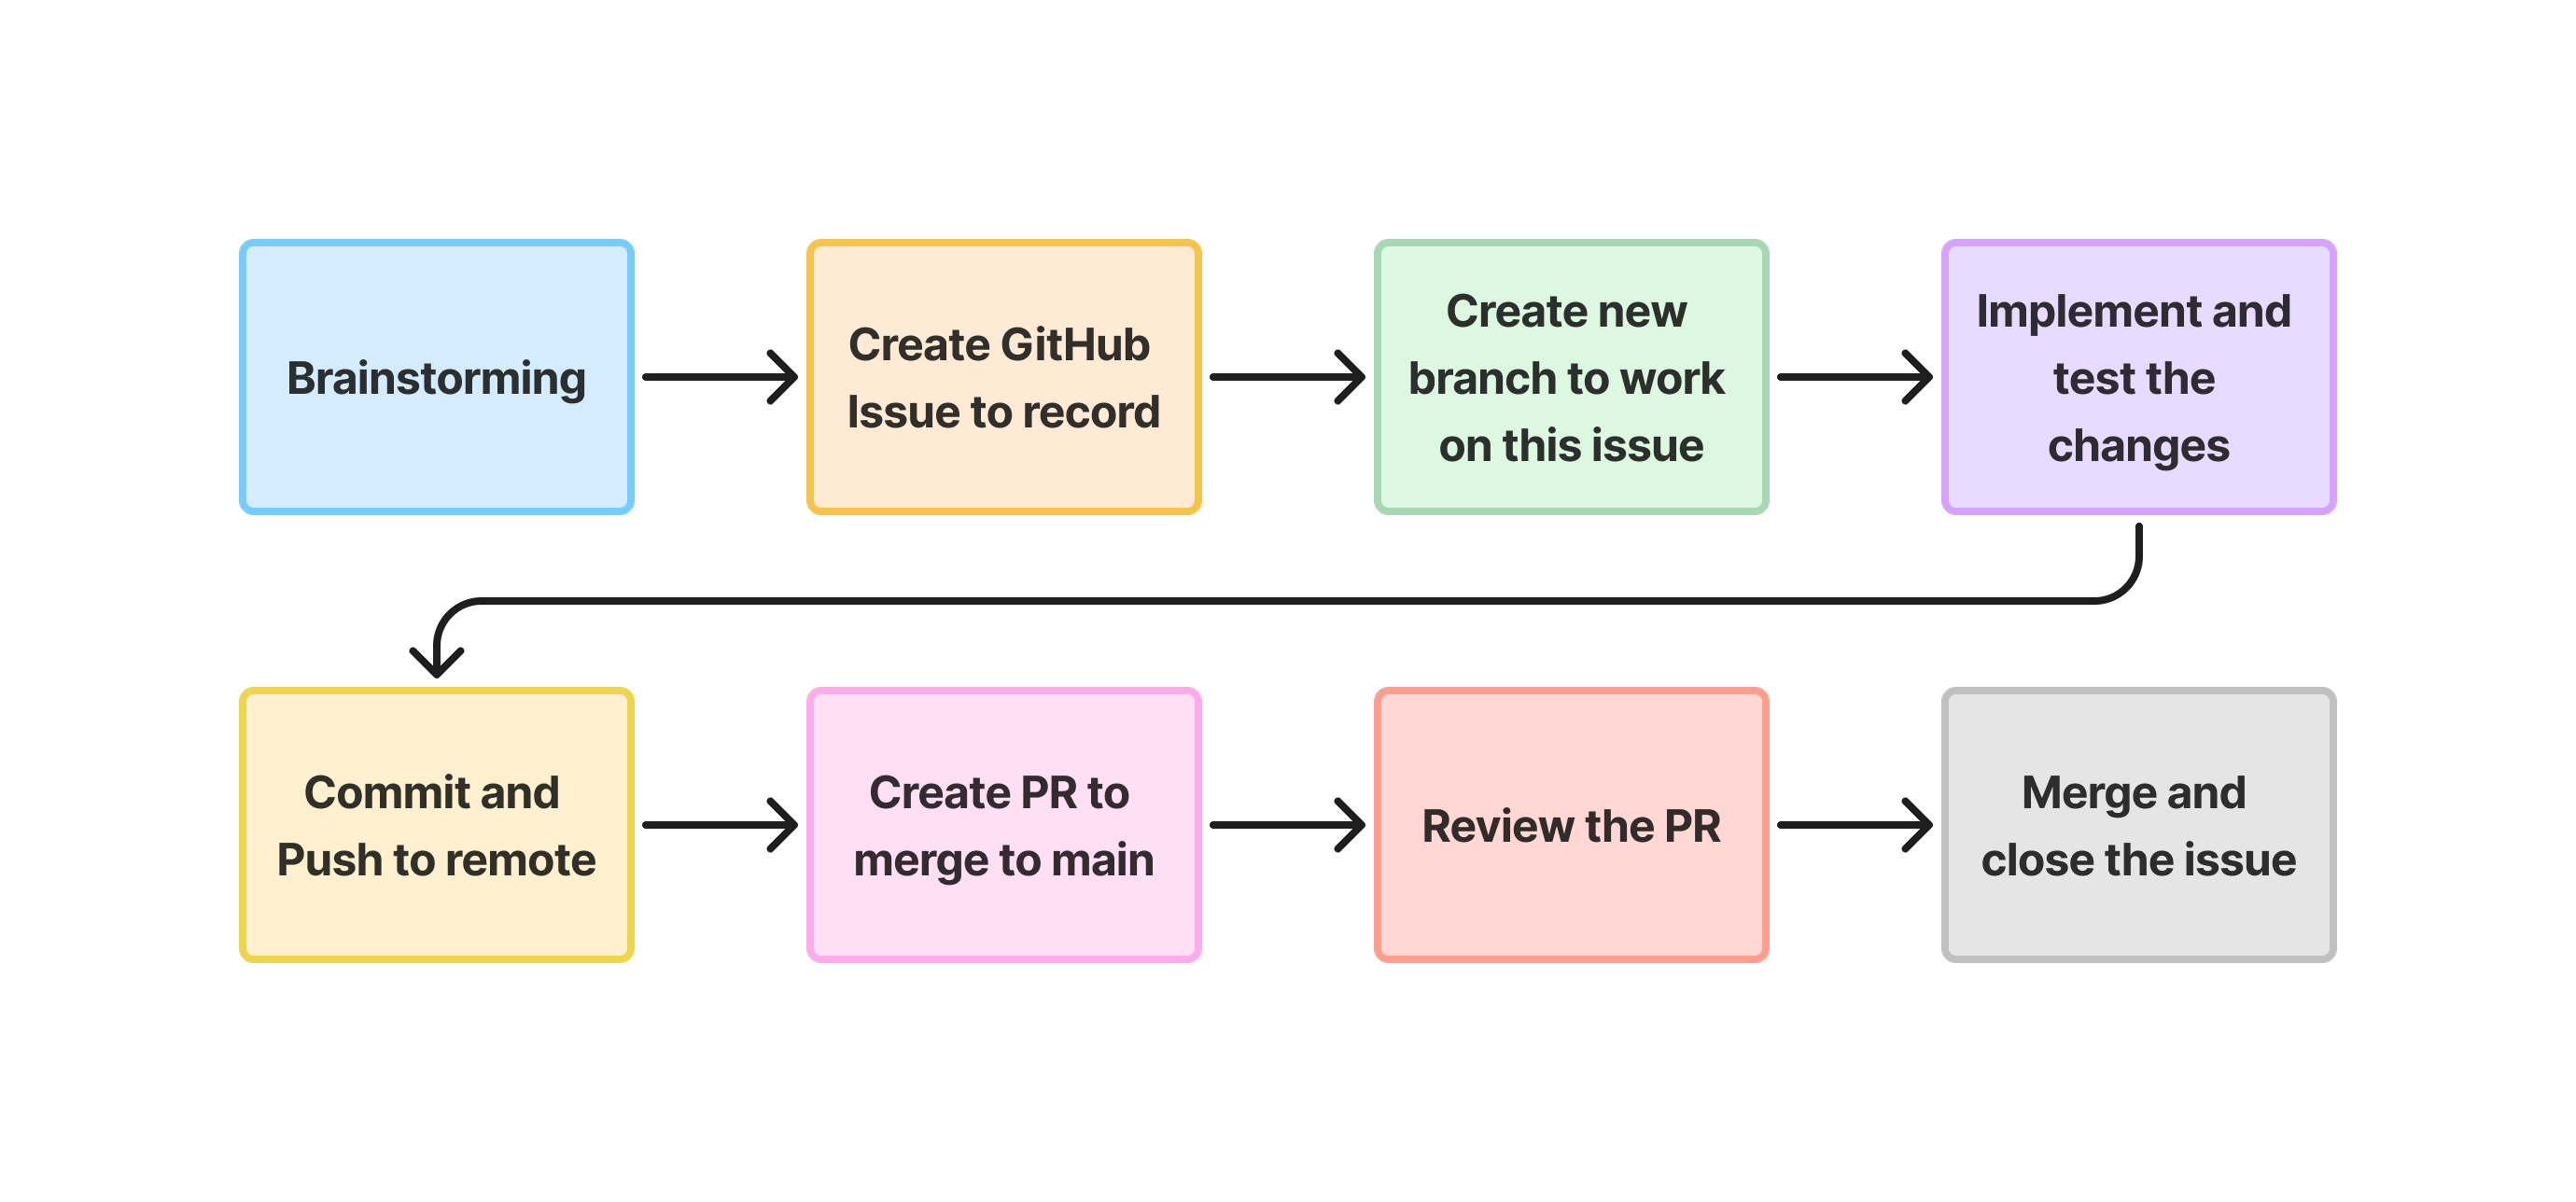
\includegraphics[width=0.9\textwidth]{figures/fig_git_workflow.png}

\end{frame}

\begin{frame}

\begin{itemize}

\item \textbf{Best practice:} Redo tasks instead of editing when needed (from Anthropic)
\begin{itemize}
\item This workflow ensures everything is properly checked
\item Clean implementation from the start
\end{itemize}

\item \textbf{Everything is recorded and traceable}
\begin{itemize}
\item Great for collaboration and knowledge sharing
\item Clear history of all changes and decisions
\end{itemize}

\item \textbf{GitHub CLI integration}
\begin{itemize}
\item Claude Code handles all GitHub operations via \texttt{gh} CLI
\item No need to learn GitHub commands — just prompt what you want
\end{itemize}

\end{itemize}

\end{frame}

\begin{frame}{Worktrees for Parallel Development}

\begin{itemize}
\item \textbf{What are worktrees?}
\begin{itemize}
\item Git feature that creates linked working directories
\item Each worktree has its own branch and working state
\end{itemize}

\item \textbf{Perfect for parallel development}
\begin{itemize}
\item No need to stash or commit when switching tasks
\item Test multiple features side-by-side
\end{itemize}

\item \textbf{Claude Code + Worktrees}
\begin{itemize}
\item Let agents work on different features in parallel
\item Handle urgent fixes without disrupting current work
\item Avoid conflicts for Claude Code sessions
\end{itemize}
\end{itemize}
\end{frame}

\begin{frame}
\large
\begin{itemize}
\setlength{\itemsep}{0.4cm}
\item New features release almost every week
\item Continuously update tools, workflows, and expertise
\item Experiment with novel AI-driven methods to accelerate research
\end{itemize}
\end{frame}

\begin{frame}

\vspace{2cm}
\centering
\Huge
\textbf{Questions \& Discussion}

\end{frame}


% \bibliographystyle{unsrt}
%\bibliography{ref}
\end{document}